\documentclass{IEEEtran}
\usepackage{graphicx}
\usepackage{amsmath}

\graphicspath{{./figures/}}

% \title{Integrating 3D Localization and Haptic Feedback for Interactive Graphics Manipulation}
% \title{Integrating 3D Localization, Haptic Devices, and Head Mounted Devices for Virtual Reality}
% \title{General Platform for Interactive Graphics Manipulation with Haptic Feedback via Large Scale Motion Capture}
\title{A General Platform for Immersive Virtual Reality and Interactive Manipulation with Haptic Feedback via Motion Capture}

\author{
    \IEEEauthorblockN{Armon Shariati} \\
\IEEEauthorblockA{Lehigh University \\ University of Pennsylvania}
}

\begin{document}
\setlength{\pdfpagewidth}{8.5in}
\setlength{\pdfpageheight}{11 in}
\maketitle

\begin{abstract}
    Most virtual reality systems generally fall into one of two categories:
    graphics oriented - which focus on developing immersive environments but
    generally fail to provide users with a strong sense of interactity - and
    haptics oriented - which focus on constructing tools for touch-based
    manipulation and auditory interaction but tend to be very specialized and
    exist in tightly bound device ecosystems. I present an approach for
    creating immersive graphical settings with a high degree of interactive
    manipulation using any number of haptic devices.
\end{abstract}

\section{Introduction}
\label{sec:introduction}

Virtual reality has commanded the attention of the media and the public for
decades, and in recent years the serious attention of researchers worldwide.
French playwright Antonin Artaud is first credited for coining the term
``virtual reality'' in his 1938 book \emph{The Theater and Its Double}. He uses
the term to describe theater, whereby it is a reality that is both illusory and
purely fictitious \cite{website:popularizeVR}. Technology has a come a long way
since Artuad, and our means for creating such extensional realities are ever
expanding. The allure of VR, in the contemporary sense, according to Michael
Abrash of Valve, is that ``presence is an incredibly powerful sensation, and
it's unique to VR; there is no way to create it in any other medium''
\cite{website:steampowered}.  Many devices over the years try to impart the
feeling of presence, but to do so is no trivial task. However, while VR has
long been not much more than an elusive science fiction, recent advancements in
hardware and computing power elevate its prospects to an attainable and
not-so-distant future. 

Gaming is the most obvious example of where VR might find application, and
consequently receives the most attention.  The ability to create immersive
amenable worlds which are a direct extension of our own environments are seen
to yield significant applications medicine and defense as well, among others.
In a recent study at the Department of Surgery at Yale University, researchers
found that surgical residents who receive VR training for laparoscopic
cholecystectomy are able to perform gallbladder dissections 29\% faster than
the control group. Furthermore, non-VR-trained residents are nine times more
likely to transiently fail to make progress and five times more likely to
injure the gallbladder \cite{seymour2002virtual}.

The United States military uses fully immersive virtual simulation training
systems for soldiers in Fort Bragg, N.C. \cite{website:army}. They found that
``the ability to train with this system allows the ``reset'' time to be cut
down, which allows the ability to get more repetitions in a shorter amount of
time and the ability to review each mission on a television screen to enhance
the after action review process upon completion of each mission''.  The VR
system lends itself to having a mutable nature as well. ''The Semi-Automated
Forces Works station gives the trainer the option to create additional static
items like furniture and buildings or items that are animated such as dogs and
birds, inside the virtual world. There can also be modifications made during
the scenario like adding an improvised explosive device or more vehicles and
combatants.''

Head mounted devices (HMDs), grew to become the most popular device for
delivering the VR experience for gamers.  These wearable devices track the
orientation of your head and use the measurements from their on board sensors
such as accelerometers and gyroscopes to adjust the pose of a virtual camera to
correspond to the real time movement of your head.  The first of such devices
include Nintendo's Virtual Boy, Virtual i-O i-glasses, and the VFX-1 Headgear
from Forte Tech. While all very groundbreaking for their time, they are all
plagued with the same problem as the countless HMD devices to follow, in that
the processing power can not contend with what the graphics demand.  In
addition to low resolution displays and limited communication bandwidth, the VR
experience these devices provide are limited at best and would often cause
users to feel sick after a session \cite{zachara2009challenges}. The most
contemporary versions of these devices however, show a great deal of promise.
The Oculus Rift \cite{website:oculusvr} has experienced meteoric success since
debuting in 2012; it has raised \$2.5 million in its opening kickstarter
campaign and receives praise and support from gaming giants including John
Carmack of id Software and Michael Abrash \cite{website:kickstarterovr}.
Although the attention does not go unwarranted since among the many things that
make the device so powerful, it is the first device of its kind to carefully
address the issue of tracker latency. How the Oculus does so will be explained
in Section \ref{sec:hmd}.

The progress made thus far creating visually immersive environments are
degraded if users have no robust means of interaction. Much research has
already been done developing haptic devices to interact with VR systems and
many of them are rather impressive. Examples of large commercial haptic systems
to experience great success include the CyberGrasp glove
\cite{website:cybergrasp} and the Phantom Omni \cite{website:geomagic}.
However, advanced haptic devices such as these are rarely seen interfaced with
the immersive graphical environments being developed in the game industry.
Conversely, while the gaming world focuses on developing graphic solutions, the
haptic devices used to interact with the generated scenes such as the Nintendo
Wiimote \cite{website:wiimote} are fairly one-dimensional input controllers
designed to simulate certain aspects of the experience. Although I should be
mention, that since the introduction of the Oculus, few companies have
attempted to develop more advanced haptic ancillary input and haptic devices
such as the Virtuix Omni - an omnidirectional treadmill and Razer Hydra - a
haptic controller \cite{website:razer}, they still fail to convey the same
level of interactivity as the more cutting edge devices seen in the more
general haptics field.

Ultimately, there still exists a great divide between the graphic solutions and
haptic solutions as far as integration. While some systems attempt to close the
loop from perception, to interaction, to haptic feedback, they often make it
difficult to introduce other tools into their ecosystem such as the more
advanced graphics displays. Moreover, many of these systems would also have
great difficulty providing as large of a virtual space as required for some
military applications and provide as much precision for fine manipulations
tasks such as surgical training.

I present a solution for developing immersive and interactive VR environments,
which allows developers to efficiently leverage large scale motion capture
systems in order to interface any number of haptic devices with a cutting edge
graphics pipeline, to achieve seamless interactivity between users and their
virtual realities. My design also allows my system to interface with robotic
systems as well, which could lead to interesting teleoperation and telepresence
applications. In Section \ref{sec:hmd}, I describe my usage of the Oculus as
the head mounted display. In Section \ref{sec:mocap}, I give an explanation of
how I use motion capture in my system. In Section \ref{sec:results}, I describe
the final simulation. Finally, In Section \ref{sec:future}, I outline the
direction the system should take in the future.

\section{Head Mounted Display}
\label{sec:hmd}

\begin{figure}[]
\centering
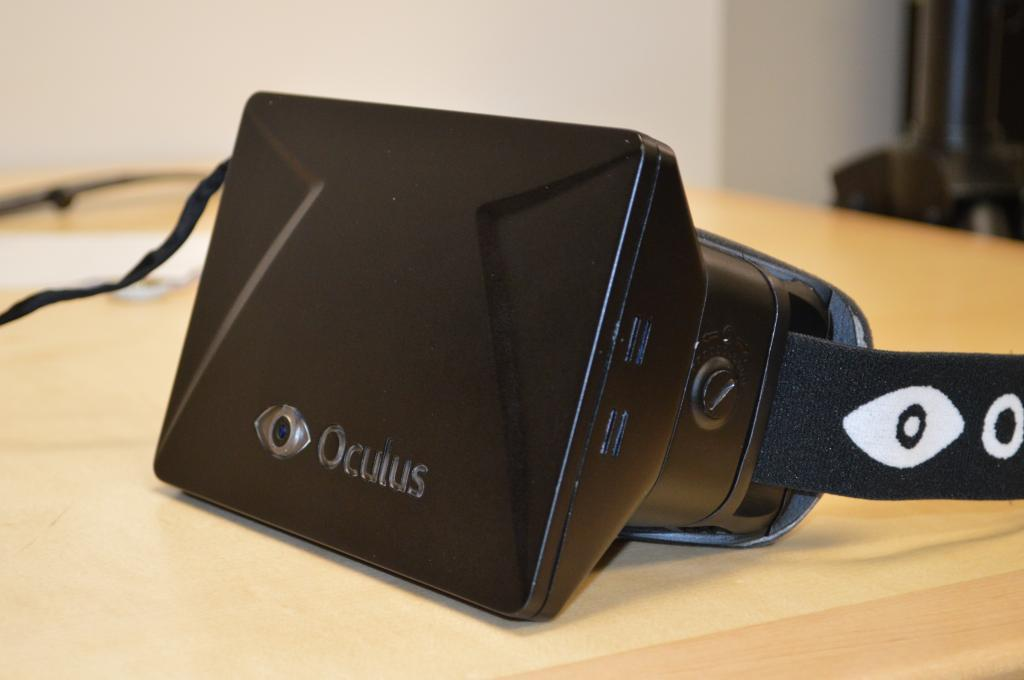
\includegraphics[width=0.5\textwidth]{oculus.jpg}
\caption{Oculus Rift Development Kit 1. 
\cite{website:pcworld}}
\label{fig:oculus}
\end{figure}

\begin{figure}[]
\centering
\includegraphics[width=0.5\textwidth]{stereo_lens.png}
\caption{Above is a stereoscopic split screen view also rendered with barrel distortion.
    Below, are the magnifying lenses of the oculus headset.
Frames displayed on the Oculus screen appear normal when the headset is worn.}
\label{fig:stereo}
\end{figure}


The Oculus Rift seen in Fig. \ref{fig:oculus} is the current state of the art
in HMD VR technology. There are several elements to the device that allow the
Oculus to provide the most immersive visual VR experience thus seen.

The first is speed.  The VR realism is directly tied to this response time and
the Oculus overcomes the problem of graphical latency, which has plagued all of
its predecessors, by sampling data from its 3-axis gyro, accelerometers, and
magnetometers at a rate of 250Hz \cite{website:roadtovr}; the newer version is
said to have a sampling rate of 1000Hz. Its ability to gather data so quickly
from its propriocetive sensors allows the graphics on the display to be
adjusted to correspond to real time head movements. Secondly, the Oculus
renders scenes split screen stereoscopic 3D. The left eye sees the left half of
the screen and the right eye sees the right half, which is consistent with
human perception. Leveraging split screen stereo greatly enhances the perceived
3D effect. Finally, the Oculus uses large magnifying lenses in order to
completely encompass the user's peripheral vision and greatly expand field of
view. All of these aspects must be considered when developing the graphics of
the scene. Fortunately the SDK provides sufficient overhead to deal with them,
allowing graphics developers to stay focused on developing graphics instead of
worrying about the details of implementation.

The most simple applications one can develop for the Oculus are created using
basic OpenGL. The only caveat being that a separate framebuffer must be bound
to the context for off-screen rendering. The framebuffer must have a texture
bound to at as well which will be written to at the last stage of the
conventional pipeline. Parameters for constructing the texture are provided
directly from the Oculus SDK programmatically. The Oculus SDK will then take the
data placed in the texture and perform the post-processing for stereoscopic 3D
rendering and distortion processing. 

Human eye pupils are approximately 65 mm apart.  This interpupillary distance
(IPD) must be taken into consideration for configuring the in-application
camera. Therefore, each scene is rendered twice, once for the virtual camera
on the left, and once for the virtual camera on the right. Both of which are
subject to a translation with respect to one another causing the stereoscopic
effect. 

The use of the large magnifying lenses causes the image succumbs to a great
deal of pincushion distortion. To rectify this distortion, the software must
apply an equal and opposite amount of barrel distortion. The final image
rendered to the Oculus's display can be seen in Fig. \ref{fig:stereo}. For the
remainder of this paper, when discussing the camera view, this refers to the
single camera model provided to the Oculus SDK before the post processing
occurs. 

However, the Oculus is not without limitations. While it is able to track
rotation effectively, it provides no means of tracking translation. Those
familiar with the company should find themselves critical, as they know that
the newer version of the Oculus does provides position tracking as well. Be
that as it may, its position tracking is limited as it is designed to track
within a small volumes, say the space in front of a desk. In addition, it
provides not ability track any other objects other than itself.

Graphics is known as the inverse problem to computer vision. Where computer
vision seeks to extract information about an environment from an image,
graphics seeks to extract information to construct an image from an
environment. What gives computer graphics the illusion of position and depth is
a mathematical process of constructing a series of transformations taking
arbitrary points from one frame of reference to another to infer position and
ultimately a projective transform to infer depth. The location of all the
particles in an object can be defined with respect to some inertial frame of
reference. If one observes the object from some alternative location and
orientation with respect to the same inertial frame, one can construct a
transformation to take points from the inertial frame to the view frame.
Ultimately, all the objects in the scene must be transformed from their own
respective frames of reference to this view frame. Manipulating the pose of
this view frame is what we are interested in. Normally, the orientation of
the Oculus is constructed from the measurements provided by its sensors,
and is used directly as the orientation of the view frame.

\begin{figure}[]
\centering
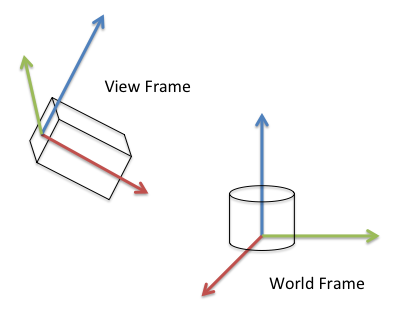
\includegraphics[width=0.5\textwidth]{world_view.png}
\caption{Two frames of reference, the view and the world. The orientation and
position of the view frame corresponds to the camera view. The axis are
defined in the graphics convention. Red is \emph{x}, green is \emph{y}, 
and blue is \emph{z}.}
\label{fig:worldview}
\end{figure}


\section{Motion Capture}
\label{sec:mocap}

\begin{figure}[]
\centering
\includegraphics[width=0.5\textwidth]{view_mask.png}
\caption{On the left is a graphical representation of the Oculus with its
tracking rig attached as well as the two different coordinate axis
corresponding to the actual graphics view, and the mask. On the right
is a picture of the Oculus as it is used in the system.}
\label{fig:mask}
\end{figure}

Motion capture systems such as the Vicon system \cite{website:vicon}, which I
chose to use in my system,  track objects through a volume by calculating 3D
spatial displacements of a set of asymmetrically mounted markers. The markers
reflect the infrared radiation emitted by LEDs which in turn is the only light
that is tracked by a set of cameras which mask out all other sources of light.
Using two or more cameras, the position of each marker can be found via
triangulation.

In order to best track the pose of the Oculus through the volume created by the
set of 6 cameras, one needs to mount the reflective markers in such a fashion
that they are difficult to occlude. To do so, I construct a simple lightweight
rig from balsa wood seen in Figure \ref{fig:mask}. I refer to the coordinate
frame associated with the rig as the mask frame. It is important to note that
the mask frame is not the same as the view frame. If orientation of the mask
frame was used for the orientation of the virtual camera, the displayed seen
would be incorrect. To account for this, I build another transformation to
take points from the mask frame to the view frame. I approximate the rotation
with the rotation matrix below.

\[
R = \begin{pmatrix} 0 & -1 & 0 \\ 0 & 0 & 1 \\ -1 & 0 & 0 \end{pmatrix}
\]

I approximate the translation between the two frames by using a ruler to
measure the distance from the point indicated as the center of the rig, and the
approximate center of the Oculus' front face.

Using a motion capture system to track position and rotation allows us to
add as many extra devices to the system, provided there are a set of markers
mounted to the device which meet the necessary criterion. For my own demo 
I chose to use a Nintendo Wiimote seen in Figure \ref{fig:wiimote}.

\begin{figure}[]
\centering
\includegraphics[width=0.5\textwidth]{wiimote.png}
\caption{Above is a Nintendo Wiimote with a set of four reflective markers
attached to its head such that it can be tracked through the motion capture
volume}
\label{fig:wiimote}
\end{figure}

\begin{figure}[]
\centering
\includegraphics[width=0.5\textwidth]{mocap.png}
\caption{This is a representation of what the different coordinate frames
look like in the system.}
\label{fig:mocap}
\end{figure}

A final representation of using motion capture to track the objects can be seen
in Figure \ref{fig:mocap}. One should note, that since now the position and
orientation of the Oculus - and in turn the view frame - is derived from the
Vicon, which establishes a world coordinate frame at a point defined on the
ground, the graphics do not exist with respect to some arbitrary world frame
defined in the graphics world, but instead they are all defined with respect to
the origin defined by the Vicon system. Furthermore, the size and position of
all graphical objects are no longer an arbitrary unit length, but are now
millimeters which is the unit reported by the Vicon. This grants developers an
extra degree of intuition because the virtual volume and all of the virtual
objects now directly correspond to space defined in the real world.



\section{Results}
\label{sec:results}

\begin{figure}[b!]
\centering
\includegraphics[width=0.5\textwidth]{reflection.png}
\caption{The trajectory of the ball incurs a reflection about the normal
vector defining the plane with which it makes contact.}
\label{fig:reflection}
\end{figure}

The test application I use to test the merit of the platform, includes three
major elements. It must provide an immersive graphical environment for the
user, interactivity with the environment, and finally some degree of haptic
feedback. The demo features a game of virtual squash. The user is placed within
a room which approximately corresponds size to the motion capture volume - 5
meters long, 2.5 meters wide, and 2.5 meters high. Alongside the user is a
paddle and ball. The pose of the paddle corresponds directly to the pose of the
Wiimote within the volume. See Figure \ref{fig:demo} for a snapshot.  When the
virtual paddle makes contact with the ball, the Wiimote vibrates, and the
paddle supplies the ball with an instantaneous velocity in the direction of the
normal vector defining the face of the paddle which made contact.  As the ball
travels, if it makes contact with any of the six faces of the bounding room or
any of the six faces of the paddle, the velocity of the ball is subject to a
reflection about the normal defining the face with which it made contact as
seen in Figure \ref{fig:reflection}. 

\[
\vec{v_{2}} = \vec{v_{1}} - 2 \frac{\vec{v_{i}} \bullet \vec{n}}{\vec{n} \bullet \vec{n}} \hat{n}
\]

Until the user chooses to reset the simulation, the ball will continue to 
bounce move about the room indefinitely.

\subsection{Software Architecture}

I built the application within the Robot Operating System (ROS) framework
\cite{website:ros}. ROS is a set of software libraries and tools that provide
``a structured communications layer above the host operating system of a
heterogeneous computing cluster'' \cite{quigley2009ros}. A ROS node publishes
the tracking data collected from the Vicon over a ROS topic which the main
graphics thread listens to. The application uses the pose of the Oculus and the
pose of the Wiimote provided by the Vicon, as the pose of the virutal camera
and virtual paddle respectively. The Vicon would provide measurements at a rate
of 100Hz. The graphics thread runs at an average rate of 60Hz, however, I
notice a sharp drop periodically down to 40Hz. The drop does not seem to affect
the rendering process greatly, but I would like to investigate the
cause\footnote{I suspect that the issue lies within communication with the
Wiimote. I naively placed the communication processes with the Wiimote within
the main graphics thread instead of making it its own process.}. The use of ROS
permits an ease of integration with many robotics platforms for teloperative
purposes, as many robotic systems are built within the ROS framework as well.

\subsection{Contact Modeling}

In order to simplify contact modeling I model the paddle as a rectangle even
though it is a rectangular prism. Therefore, two faces can really ever make
contact with the ball. The application determines contact with any face of the
room and the face of the paddle by continuously calculating the distance from
the ball to every face, and uses this set of measurements to ascertain whether
or not every point on the ball is within the bounding volume of the room and
whether or not any of the points on the ball exist on the face of the paddle.
Refer to Figure \ref{fig:normals} for an illustration of the different normals
associated with each face.

\[
D = \vec{(x - p)} \bullet \hat{n}
\]

Above, $D$ is the distance between a point and a plane; $x$ and $p$ are
the locations of a point on the plane and the point for which the calculation
is being performed, respectively.
\smallskip


\begin{figure}[]
\centering
\includegraphics[width=0.5\textwidth]{normals.png}
\caption{An illustration of the position and orientation of all the 
normals defining each face.}
\label{fig:normals}
\end{figure}

If every point on the ball is within the room, the distances between all the
points on the ball and each face of the room should be positive. If the sign of
any of the distances becomes negative, this indicates contact with the
associated face. The velocity vector of the ball then undergoes a reflection
about the normal vector affiliated with the face which makes contact.
Similarly, to determine contact with the paddle, the application determines if
any point on the ball has entered the bounding prism of the paddle. If so, the
application determines which side of our simplified face model the center of
the ball resides, and uses either the normal vector for reflection if the
center is in front of the paddle or the negative of the normal vector if the
center is behind the paddle.

\begin{figure}[]
\centering
\includegraphics[width=0.5\textwidth]{demo.png}
\caption{On the left is a single image of the environment during the simulation
which is rendered to the Oculus; notice the ball and paddle.  On the right is
the user interacting with the VR.}
\label{fig:demo}
\end{figure}

\section{Future Work}
\label{sec:future}

There are a few shortcomings of my system I would like to address as well 
as a few avenues for expansion in the future. 

The length of the wires connecting the Oculus to the desktop computer are
rather short, fettering the user with approximately 1.5 meter long tether.
Therefore, even though the generated volume has dimensions of 5 by 2.5 by 2.5
meters, the user only may move within an inscribed circle with a radius of 1.5
meters.  I would like to enable exploration of the entire volume in the future. 

Secondly, the environment the user is placed in - the virtual squash court - is
rather bland. There is no lighting or shadow. The ball, each wall of the room,
and each face of the paddle are all solid colors. Moreover, the main issue that
remains is that the environment is not very familiar to the user. I would
also like to spend more time developing more vivid and relatable scenes in order
to generate more immersive experiences. OpenGL may be sufficient, although
more sophisticated game engines such as Unity \cite{website:unity} may also
be of interest.

Finally, even though the platform is designed to support more sophisticated
haptic devices a Wiimote is the only haptic device used in the
system\footnote{Pressed for time, when there were interfacing issues with a
more advanced device, I defaulted to using a simple Wiimote.}. In the future I
would like to experiment with more advanced haptic devices and develop
simulations that would provide higher degrees of interactivity. Other
applications include, virtual sculpting, construction, and as mentioned before,
robotic teleoperation.


\section{Acknowledgements}
I would like to thank Rahul Mangharam for generously providing many of the
resources necessary for building the system. I would especially like to thank
my advisor Professor Camillo Jose Taylor and my graduate student mentor
Anthony Cowley for their tutelage. Finally, I would like extend special thanks
to Professor Katherine Kuchenbecker and Professor Max Mintz for their efforts
to organize the REU program.

\bibliographystyle{IEEEtran}
\bibliography{IEEEabrv,bibliography}

\end{document}
